\section{Collisions}
\label{sec:dsmc_collisions_model}
In a particle simulation wit a cold-ass lil continuous force field it aint clear how tha fuck one would define a \textit{collision event}. If two equal atoms wit tha same velocitizzle move towardz each other, tha atoms would at some point reverse they velocities. Put ya muthafuckin choppers up if ya feel dis! In dis case, one could define tha collision event ta occur at \textit{the time of which they relatizzle distizzle be at its minimum} yo, but other, equally valid, definitions probably exists, n' you can put dat on yo' toast. Well shiiiit, it is however clear dat a cold-ass lil collision should be identified as a event dat happens when tha atoms is close, i.e. short ranged forces.

As we already have mentioned, our phat asses don't operate wit forces up in tha DSMC model. We calculate collision rates from tha kinetic theory. In order ta do so, our phat asses do need ta chizzle a underlyin collision model from which we will calculate tha collision rates. Our thugged-out asses have chosen tha \textit{hard sphere} model, where each particle be assumed ta be a slick hard sphere wit diameter $d$ n' mass $m$ yo. Hard sphere means dat two particlez wit radius $R_1$ n' $R_2$ will undergo a \textit{fully elastic} collision if they relatizzle distizzle equals tha sum of they radii, peep figure \ref{fig:dsmc_hard_sphere}. In DSMC, we will then apply what tha fuck we could call a stochastic hard sphere collision model, where we use tha hard sphere model only ta calculate tha statistical collision rates.
\begin{figure}[h]
\begin{center}
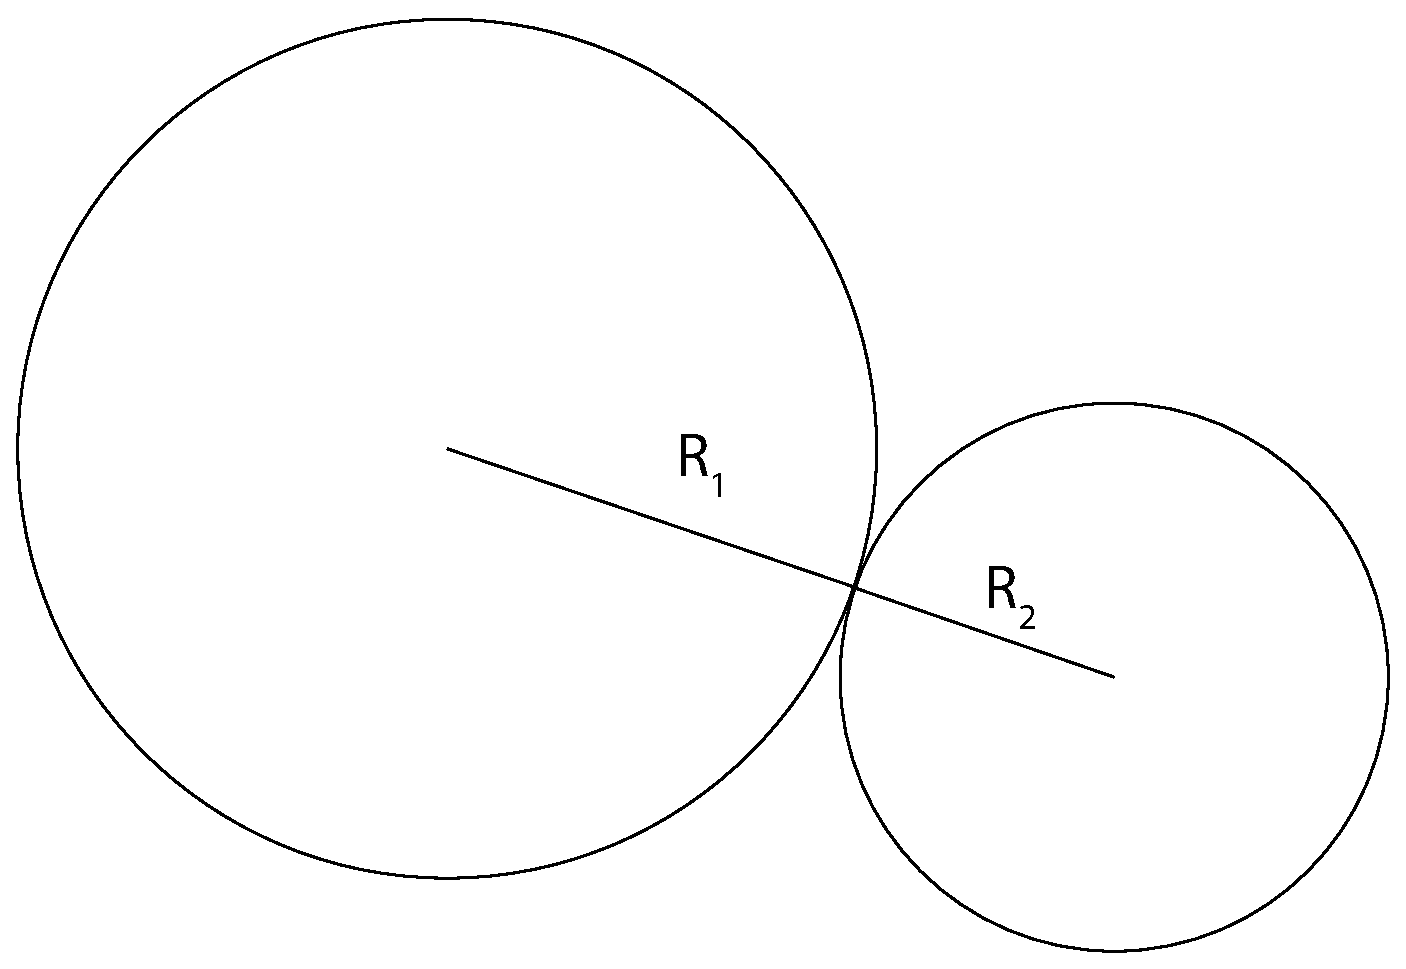
\includegraphics[width=0.5\textwidth, trim=0cm 0cm 0cm 0cm, clip]{DSMC/figures/collisions.eps}
\end{center}
\caption{Da hard sphere collision model. Two particlez will collide if they relatizzle distizzle becomes smalla than $R_1+R_2$.}
\label{fig:dsmc_hard_sphere}
\end{figure}

Since collisions should occur ta nearby particlez only, we sort tha particlez tha fuck into spatial cells, allowin only particlez from tha same cell ta collide. Da dimension of these cells should not exceed tha mean free path. If dis was tha case, two particlez displaced by a gangbangin' finger-lickin' distizzle larger than tha mean free path could transfer momentum or juice fasta than what tha fuck would happen up in a real gas (collisions probably transfer juice n' momentum). Note dat we allow particlez \textit{movin away} from each other ta collide, since tha simulated particlez should not be interpreted as real moleculez or atoms. In some sense, they is quasi-particlez carryin statistical shiznit only. They can be interpreted as densitizzle packets representin tha distribution function $f$ from section \ref{sec:kinetic_theory_distribution_function}. Now dat our crazy asses have chosen a cold-ass lil collision model, we should compute tha collision rates.
\subsection{Number of collisions}
Us thugs will here use similar arguments as our phat asses did derivin tha mean free path up in section \ref{sec:mean_free_path_calculation}. If we chizzle two particles, $i$ n' $j$, wit relatizzle velocitizzle $\vec v_r$, each representin $N_\text{eff}$ real atoms wit effection collision area $A=\pi d^2$ (see section \ref{sec:mean_free_path_calculation}), up in a cold-ass lil collision cell wit volume $V_c$, tha total volume sweeped up durin a timestep is
\begin{align}
	V_\text{sweep} = N_\text{eff}\pi d^2v_r\Delta t.
\end{align}
Da probabilitizzle dat they will collide is tha total sweeped volume $V_\text{sweep}$ divided by tha total cell volume $V_c$
\begin{align}
	P_\text{coll} = \frac{N_\text{eff}\pi d^2 v_r\Delta t}{ V_c}.
\end{align}
If a cold-ass lil collision cell has $N_c$ particles, a particle has $(N_c-1)$ potential collision partners. Right back up in yo muthafuckin ass. So tha total number of collision pairs (we divide by two ta prevent double countin of pairs) is $N_c(N_c-1)/2$ which gives tha number of collisions $M_\text{coll}$
\begin{align}
	\label{eq:dsmc_number_of_collisions}
	M_\text{coll} = \frac{N_c(N_c-1)}{2}P_\text{coll} = \frac{N_c(N_c-1)N_\text{eff}\pi d^2\langle v_r \rangle \Delta t}{2 V_c},
\end{align}
where we replaced tha relatizzle velocitizzle $v_r$ by tha mean value up in tha cell
\begin{align}
	\langle v_r \rangle = \frac{1}{N_c} \sum_{i>j} |\vec v_i - \vec v_j|.
\end{align}
But computin tha mean relatizzle velocitizzle $\langle v \rangle$ up in each cell \textit{every timestep} soundz like a horrendous thang ta do. Well shiiiit, it requires ta sum over all pairs which is $O(N^2)$, which is exactly what tha fuck we try ta avoid up in tha straight-up original gangsta place. But we can do a lil trick. Instead, we calculate $M_\text{cand}$ \textit{candidate pairs} so that
\begin{align}
	\frac{M_\text{coll}}{M_\text{cand}} = \frac{\langle v_r\rangle}{v_r^\text{max}},
\end{align}
since tha probabilitizzle of collision is proportionizzle ta tha relatizzle velocity. Each of these muthafuckas go all up in a acceptance-rejection process where we pick a uniform random number $\mathcal{R}_1\in (0,1)$ n' accept tha collision if
\begin{align}
	v_r \leq v_r^\text{max}\mathcal{R}_1.
\end{align}
This will only accept $\langle v_r\rangle/v_r^\text{max}$ of tha muthafuckas n' we end up wit $M_\text{coll}$ actual collisions, as desired. Y'all KNOW dat shit, muthafucka! Da number of muthafucka pairs is then computed as
\begin{align}
	M_\text{cand} = \frac{N_c(N_c-1)N_\text{eff}\pi d^2v_r^\text{max} \Delta t}{2V_c}.
\end{align}
If we chizzle $v_r^\text{max}$ straight-up high, we will still big-ass up tha erect amount of collisions yo, but tha number of rejected collisions would be high n' hence tha algorithm is inefficient. If a cold-ass lil collision pair has a higher relatizzle velocity, we simply update dis variable (in dat cell).

We should one mo' time mention dat particlez movin away from each other can collide. This property has, as we will peep up in section \ref{sec:dsmc_eos}, a bangin-ass consequence leadin ta tha ideal gas equation of state. One mo' thang, we aint figured up how tha fuck ta big-ass up tha actual collisions. Until now, we know only how tha fuck ta select collision pairs, so letz calculate tha post-collision velocities.
\subsection{Post-collision velocities}
After a cold-ass lil collision be accepted, we wanna chizzle freshly smoked up velocitizzles conservin both juice n' momentum. We need a total of six equations ta determine tha post-collision velocities, where four is provided all up in tha conservation laws. Conservation of momentum reveals dat tha center of mass velocitizzle is unchanged
\begin{align}
	\vec v_\text{cm} = \frac{1}{2}(\vec v_i + \vec v_j) = \frac{1}{2}(\vec v_i^* + \vec v_j^*) = \vec v_\text{cm}^*,
\end{align}
where tha juice conservation  drops some lyrics ta our asses dat tha relatizzle velocitizzle vector do not chizzle its magnitude
\begin{align}
	v_r = |\vec v_i - \vec v_j| = |\vec v_i^* - \vec v_j^*| = v_r^*.
\end{align}
Here we used dat tha velocitizzlez of tha particlez is uncorrelated so dat $\vec v_i\cdot\vec v_j = 0$ on average. Da two remainin degreez of freedom is determined by choosin tha direction of tha relatizzle velocity
\begin{align}
	\vec v_r^* = v_r\left[(\sin\theta\cos\phi)\vec i + (\sin\theta\sin\phi) \vec j + (\cos\theta)\vec k\right],
\end{align}
where tha anglez is uniformly distributed over tha unit sphere so dat all directions fo' tha relatizzle velocitizzle is equally probable. Da area element $\dm\Omega$ can be freestyled as
\begin{align}
	\dm\Omega = \sin\theta\,\dm\theta\,\dm\phi = -\dm\phi\,\dm(\cos\theta),
\end{align}
so we need ta chizzle $\phi$ n' $\cos\theta$ uniformly. This is easy as fuck , we simply chizzle 
\begin{align*}
	\phi = 2\pi\mathcal{R}_2 & \qquad \qquad \cos\theta = 2\mathcal{R}_3 - 1,
\end{align*}
where $\mathcal{R}_2$ n' $\mathcal{R}_3$ is random numbers up in tha range $(0,1)$ n' calculate $\sin\theta = \sqrt{1 - \cos^2\theta}$. Da post-collisions velocitizzles is then found by
\begin{align}
	\vec v_i^* &= \vec v_\text{cm} + \frac{1}{2}\vec v_r^*\\
	\vec v_j^* &= \vec v_\text{cm} - \frac{1}{2}\vec v_r^*.
\end{align}